\documentclass[10pt]{article}
\usepackage{graphicx}
\usepackage{geometry}
\usepackage{color}

\geometry{
  paper=a4paper,
  margin=27pt,
  includeheadfoot
}
\graphicspath{{images/}}

\title{My first LaTeX document}
\author{LI Lunlong\thanks{Supervised by Wang Zhe and JU Yi for this paper.}}
\date{July 2023} % if omitted, the date will be the current date of compiling

\begin{document}

\maketitle
We have now added a title, author and date to our first \LaTeX{} document!
The following is a figure produced in the study of this essay. 
It illustrates the optimization performance and control behaviors of MPC \(Model Predictive Control\)
and RBC \(Rule Based Control\).
\begin{figure}[h] % h means show the figure inline rather than floating in another page
    \centering
    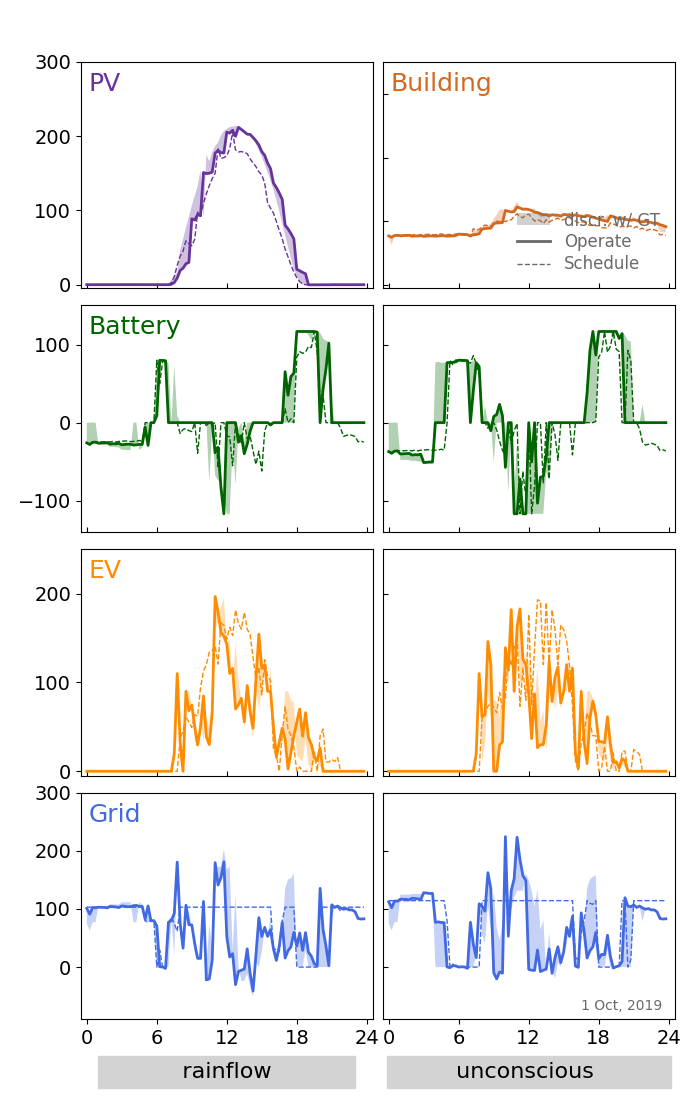
\includegraphics[width=0.4\textwidth]{case1}
    \caption[short]{The control performance of MPC and RBC}
    \label{fig:case1}
\end{figure}

\textbf{The following paragraphs implement different text styles and rules:}
\begin{itemize}
    \item \textcolor{blue}{$\backslash$textbf$\{$text$\}$}: This command makes \textbf{bold text}.
    \item \textcolor{blue}{$\backslash$textit$\{$text$\}$}: This command applies \textit{italics sytle}.
    \item \textcolor{blue}{$\backslash$underline$\{$text$\}$}: This command applies \underline{underline sytle}.
    \item Cascading commands combine different styles: \textbf{\textit{\underline{Bold+italics+underline}}}
    \item Another useful command is \textcolor{red}{$\backslash$emph$\{$text$\}$}, which automaticly decides the text style depending on the context: \\
          The movie Dead Poets Society is widely spread by \emph{"Carpe diem"}, a Latin adage means seize the day.\\
          \textit{The movie Dead Poets Society is widely spread by \emph{"Carpe diem"}, a Latin adage means seize the day.}\\
          \textbf{The movie Dead Poets Society is widely spread by \emph{"Carpe diem"}, a Latin adage means seize the day.}\\
          \underline{The movie Dead Poets Society is widely spread by \emph{"Carpe diem"}, a Latin adage means seize the day.}\\
\end{itemize}

\textbf{ The following part is a brief introduction to the principles and algorithms of XGBoost:}

Some math expressions:
\begin{itemize}
  \item $\hat{y}_i^{(T)}=\sum_{i=1}^{T} f_j(x_i)$
\end{itemize}


\end{document}